\newpage
\chapter{Project Logic Diagrams}
\label{ch-diagrams}

In a large project such as the Design Synthesis Exercise, a planning and task division have to be made and followed to keep the design process organised. The diagrams created in the Project Plan in the beginning of the project have been revised and more detail for the second halve of the project is added. In \autoref{fig:organigram} the organigram of the team can be found. 



\begin{figure}[h]
    \centering
    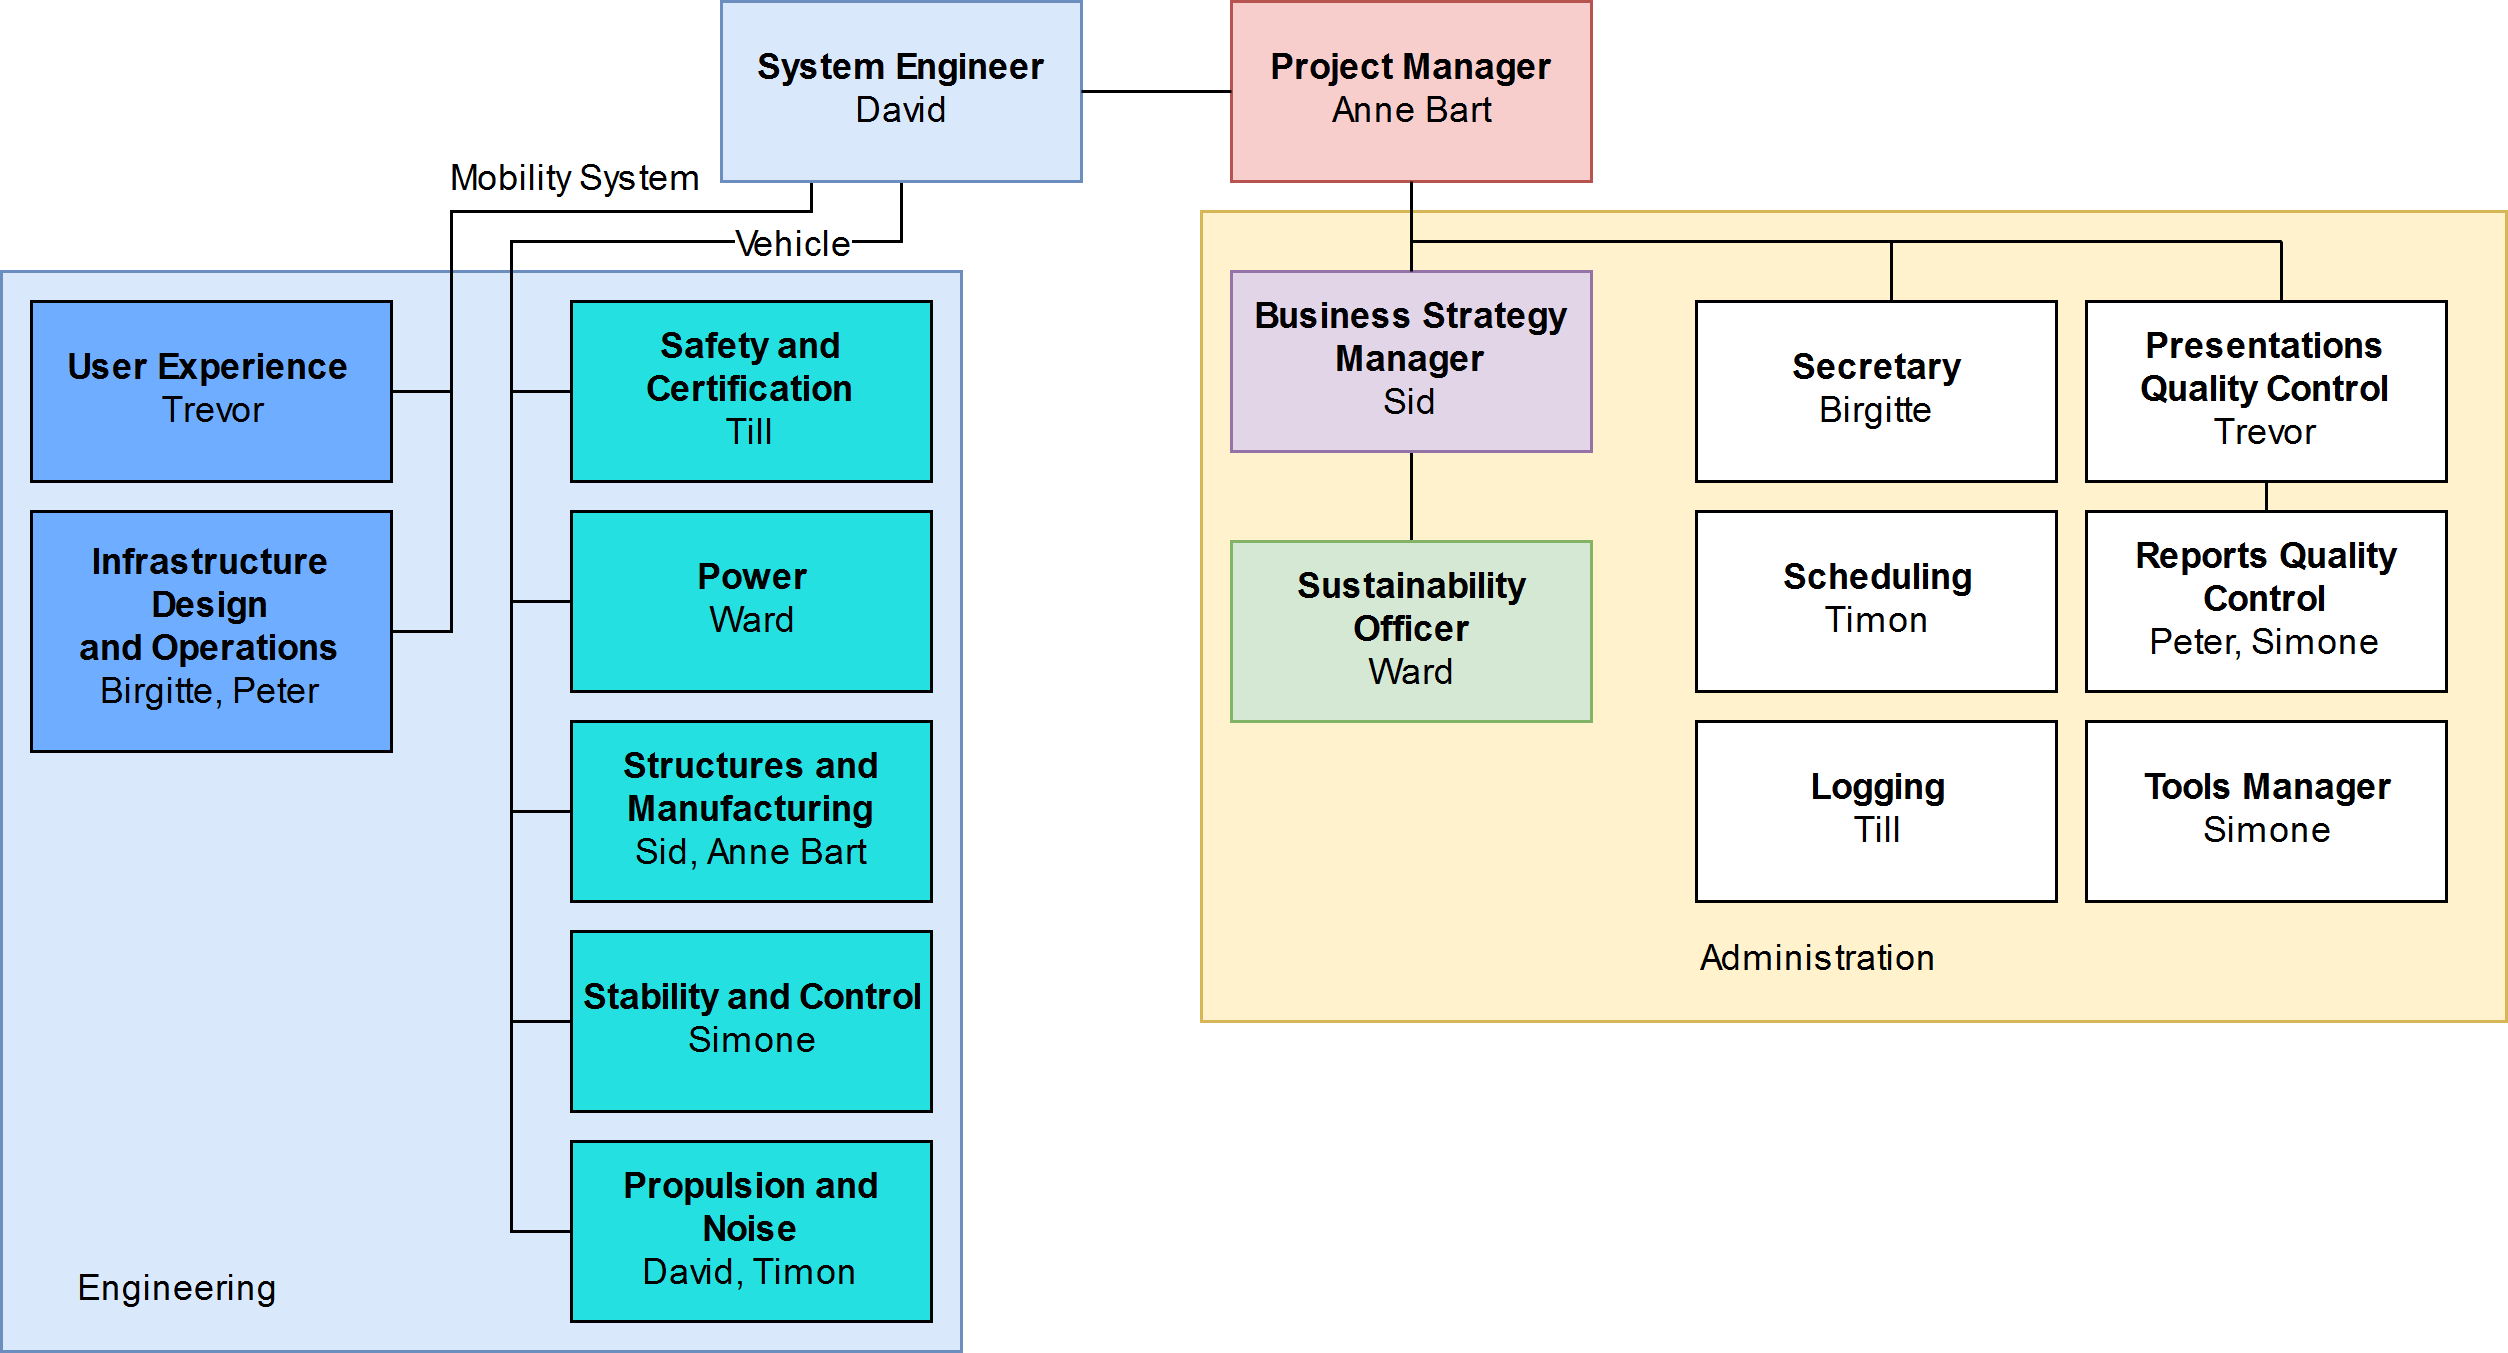
\includegraphics[width=0.9\linewidth]{Figures/organigram.png}
    \captionsetup{justification=centering}
    \caption{Team organigram}
    \label{fig:organigram}
\end{figure}



The updated Work Flow Diagram can be found on the foldout on page 64. The structure of the Midterm and Final part of the project is revised and also worked out in the Work Breakdown Structure (page 65). In the included diagrams, all tasks are given identifiers. The first initials indicate the phase, followed by the deliverable number. After the hyphen, Work Packages (WP) are given a number and tasks a letter. Generally a WP should contain 2-7 tasks and each task takes from 1 to 8 hours to complete without interruption. The labelling convention is the following: $\underbrace{\text{BR}}_\text{Phase}\underbrace{01}_\text{Deliverable ID}-\underbrace{02}_\text{WP ID}\underbrace{A}_\text{Task ID}$ 

Finally, the Gantt Chart for the second halve of the project is shown on pages 66 and 67.

%\begin{figure}[htbp]
%  \centering
%  \includesvg{Figures/WFD_Final_Phase.svg}
%  \caption{svg image}
%\end{figure}

%\includepdf[pages={1},fitpaper]{Figures/WFD_Final_Phase.pdf}


%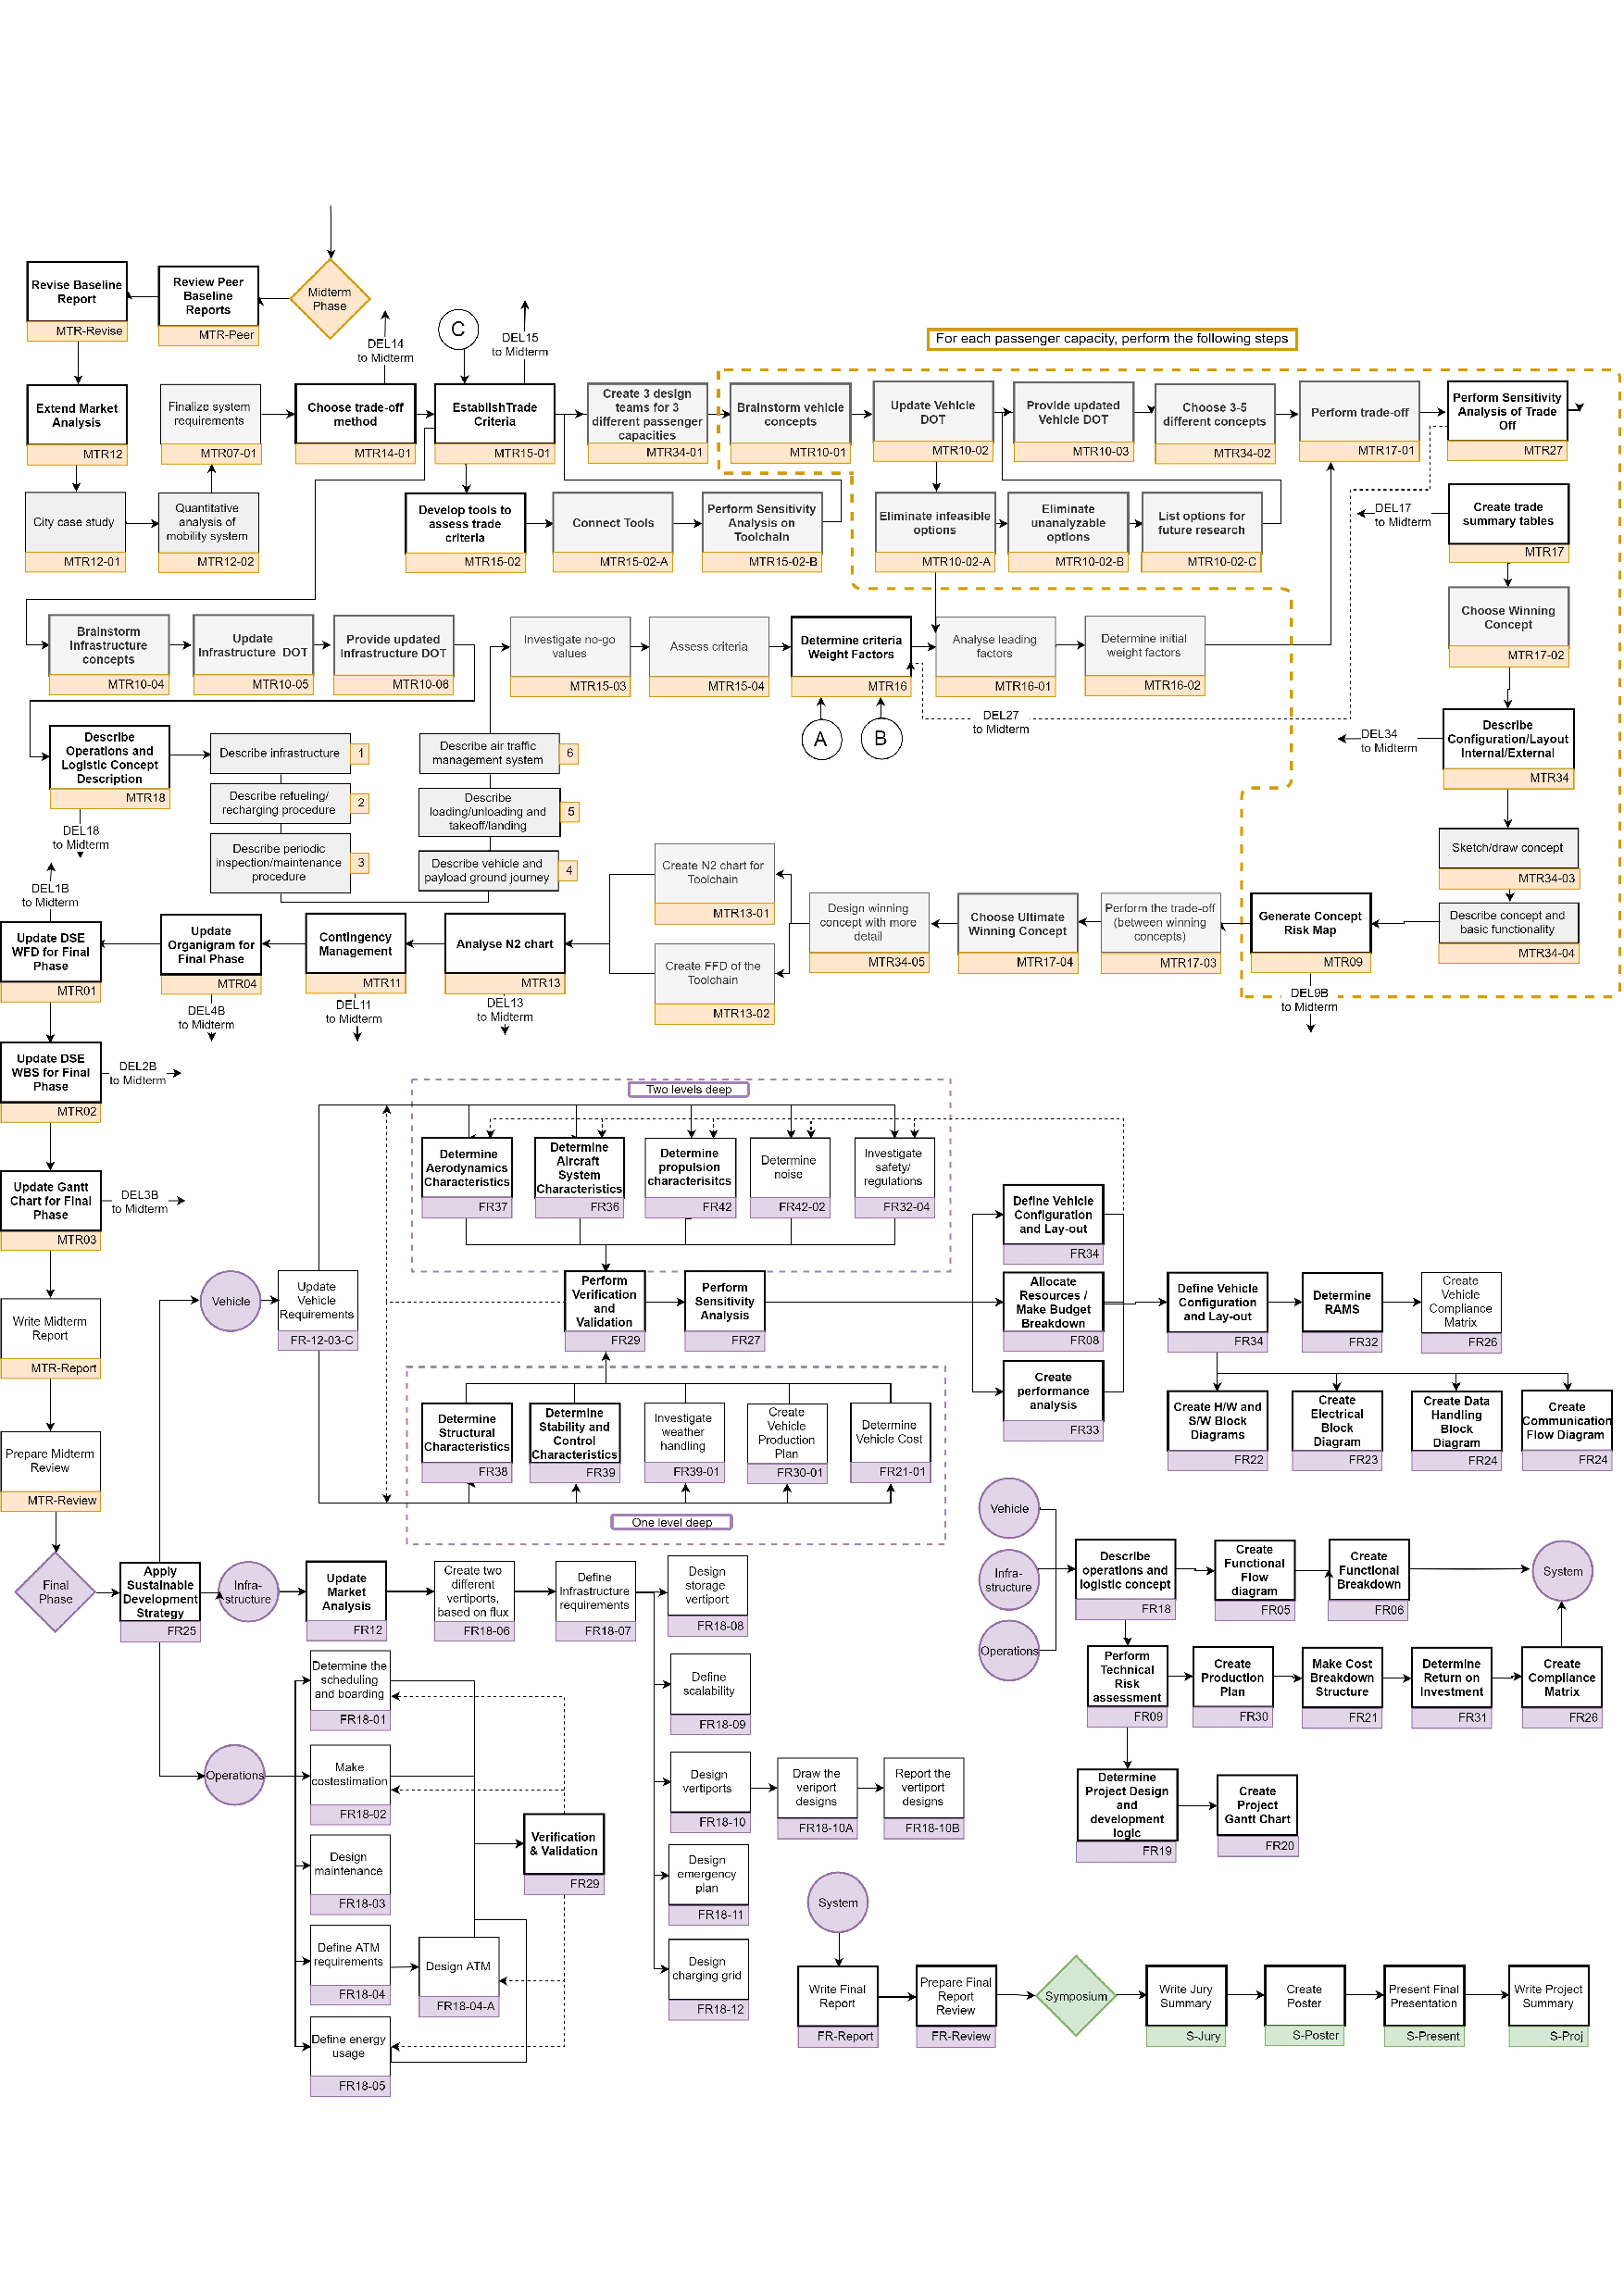
\includepdf[pages={1},fitpaper]{Figures/WFD_Final.pdf}
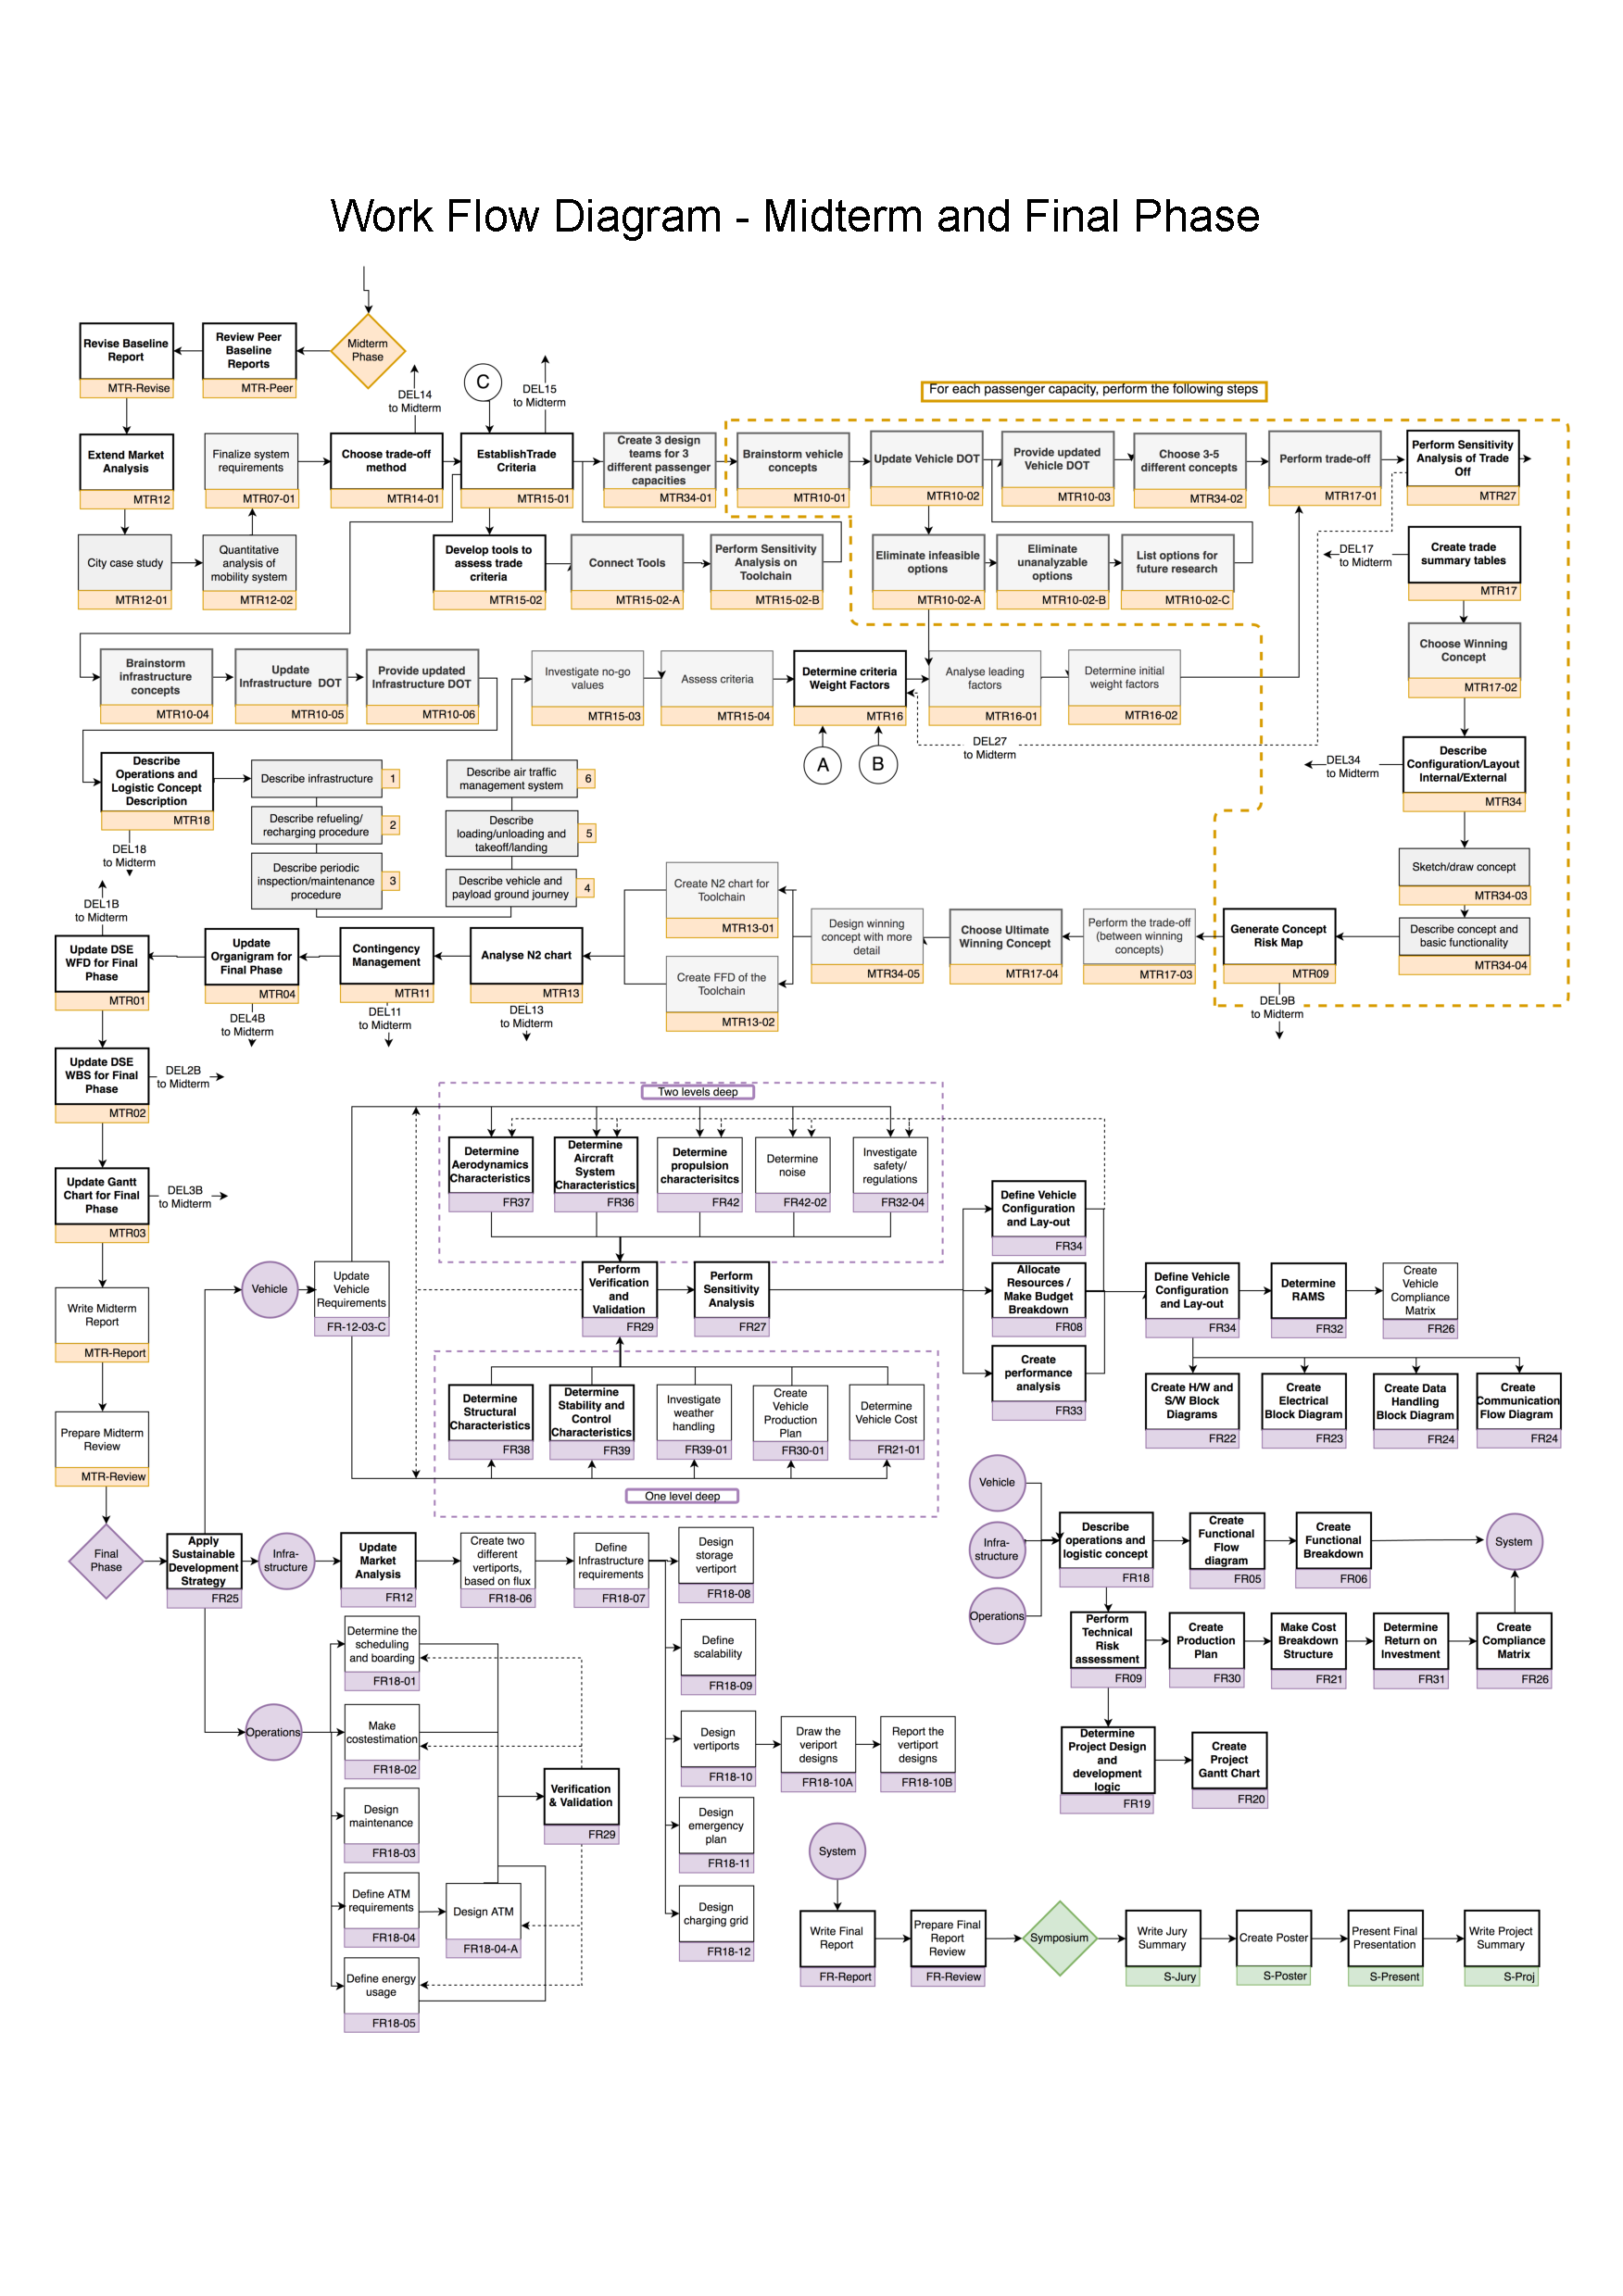
\includepdf[pages={1},fitpaper]{Figures/WFDFinalPhase.pdf}
%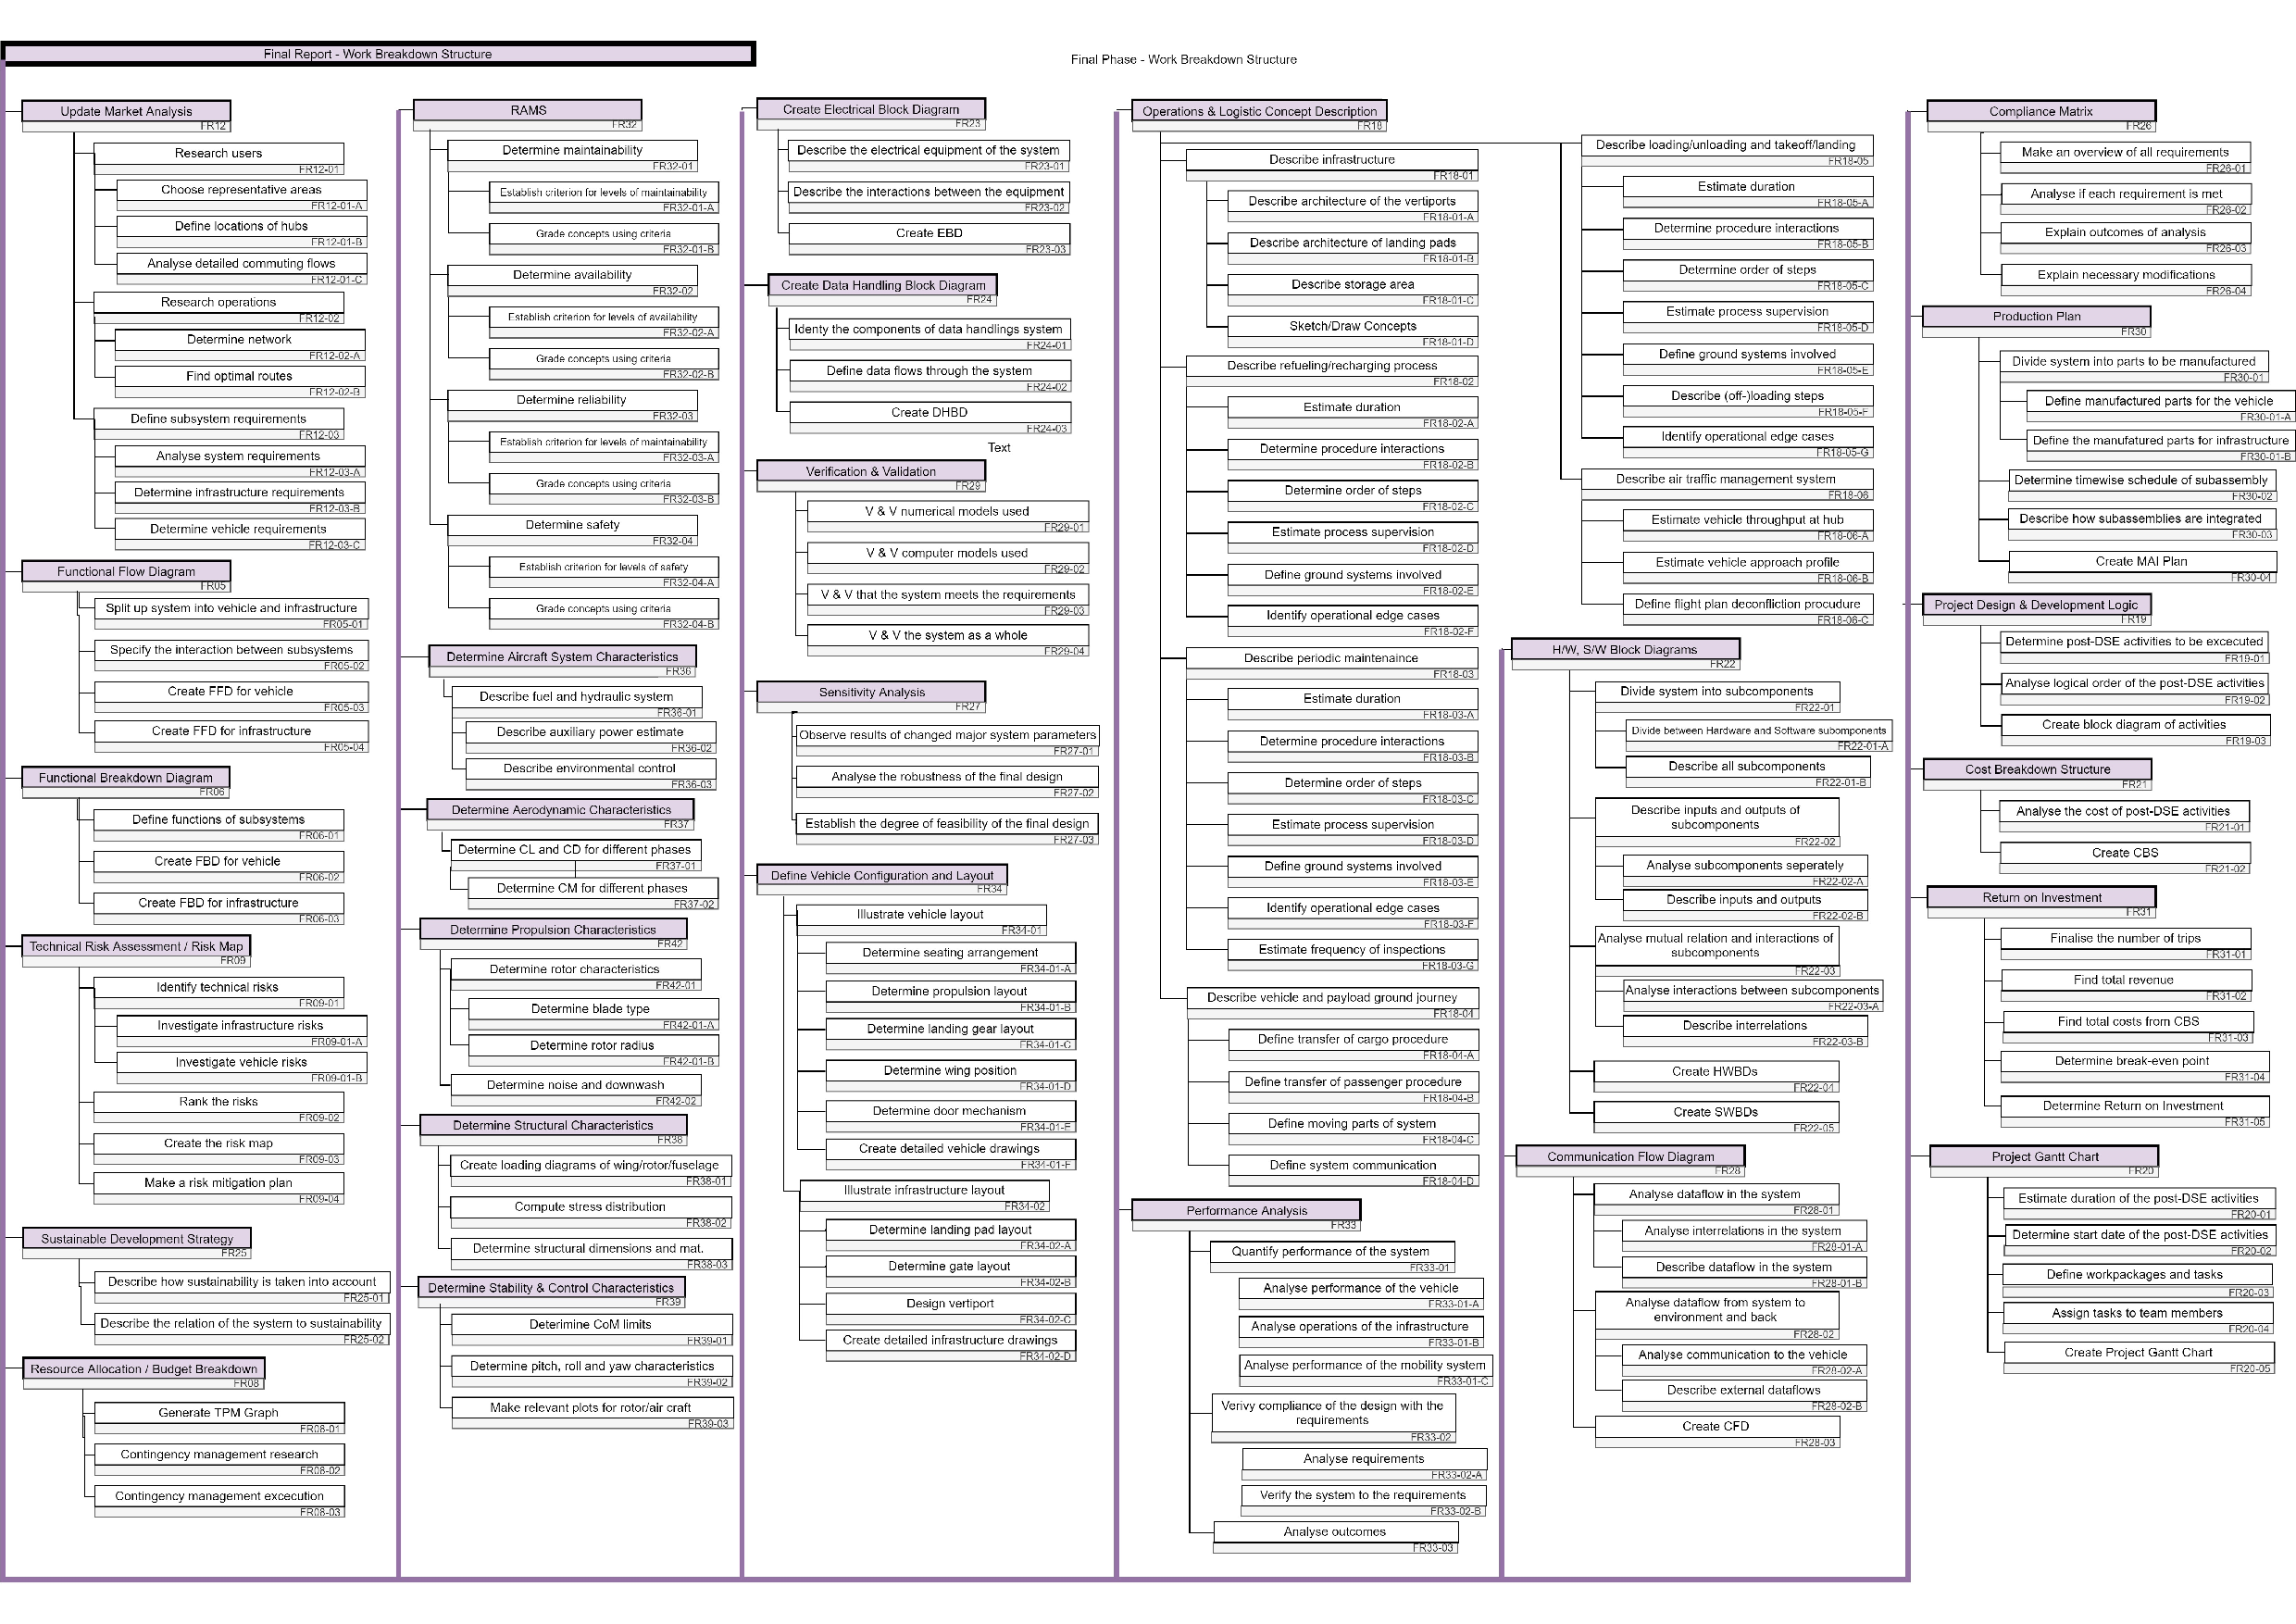
\includepdf[pages={1},fitpaper]{Figures/WBS_MTR.pdf}
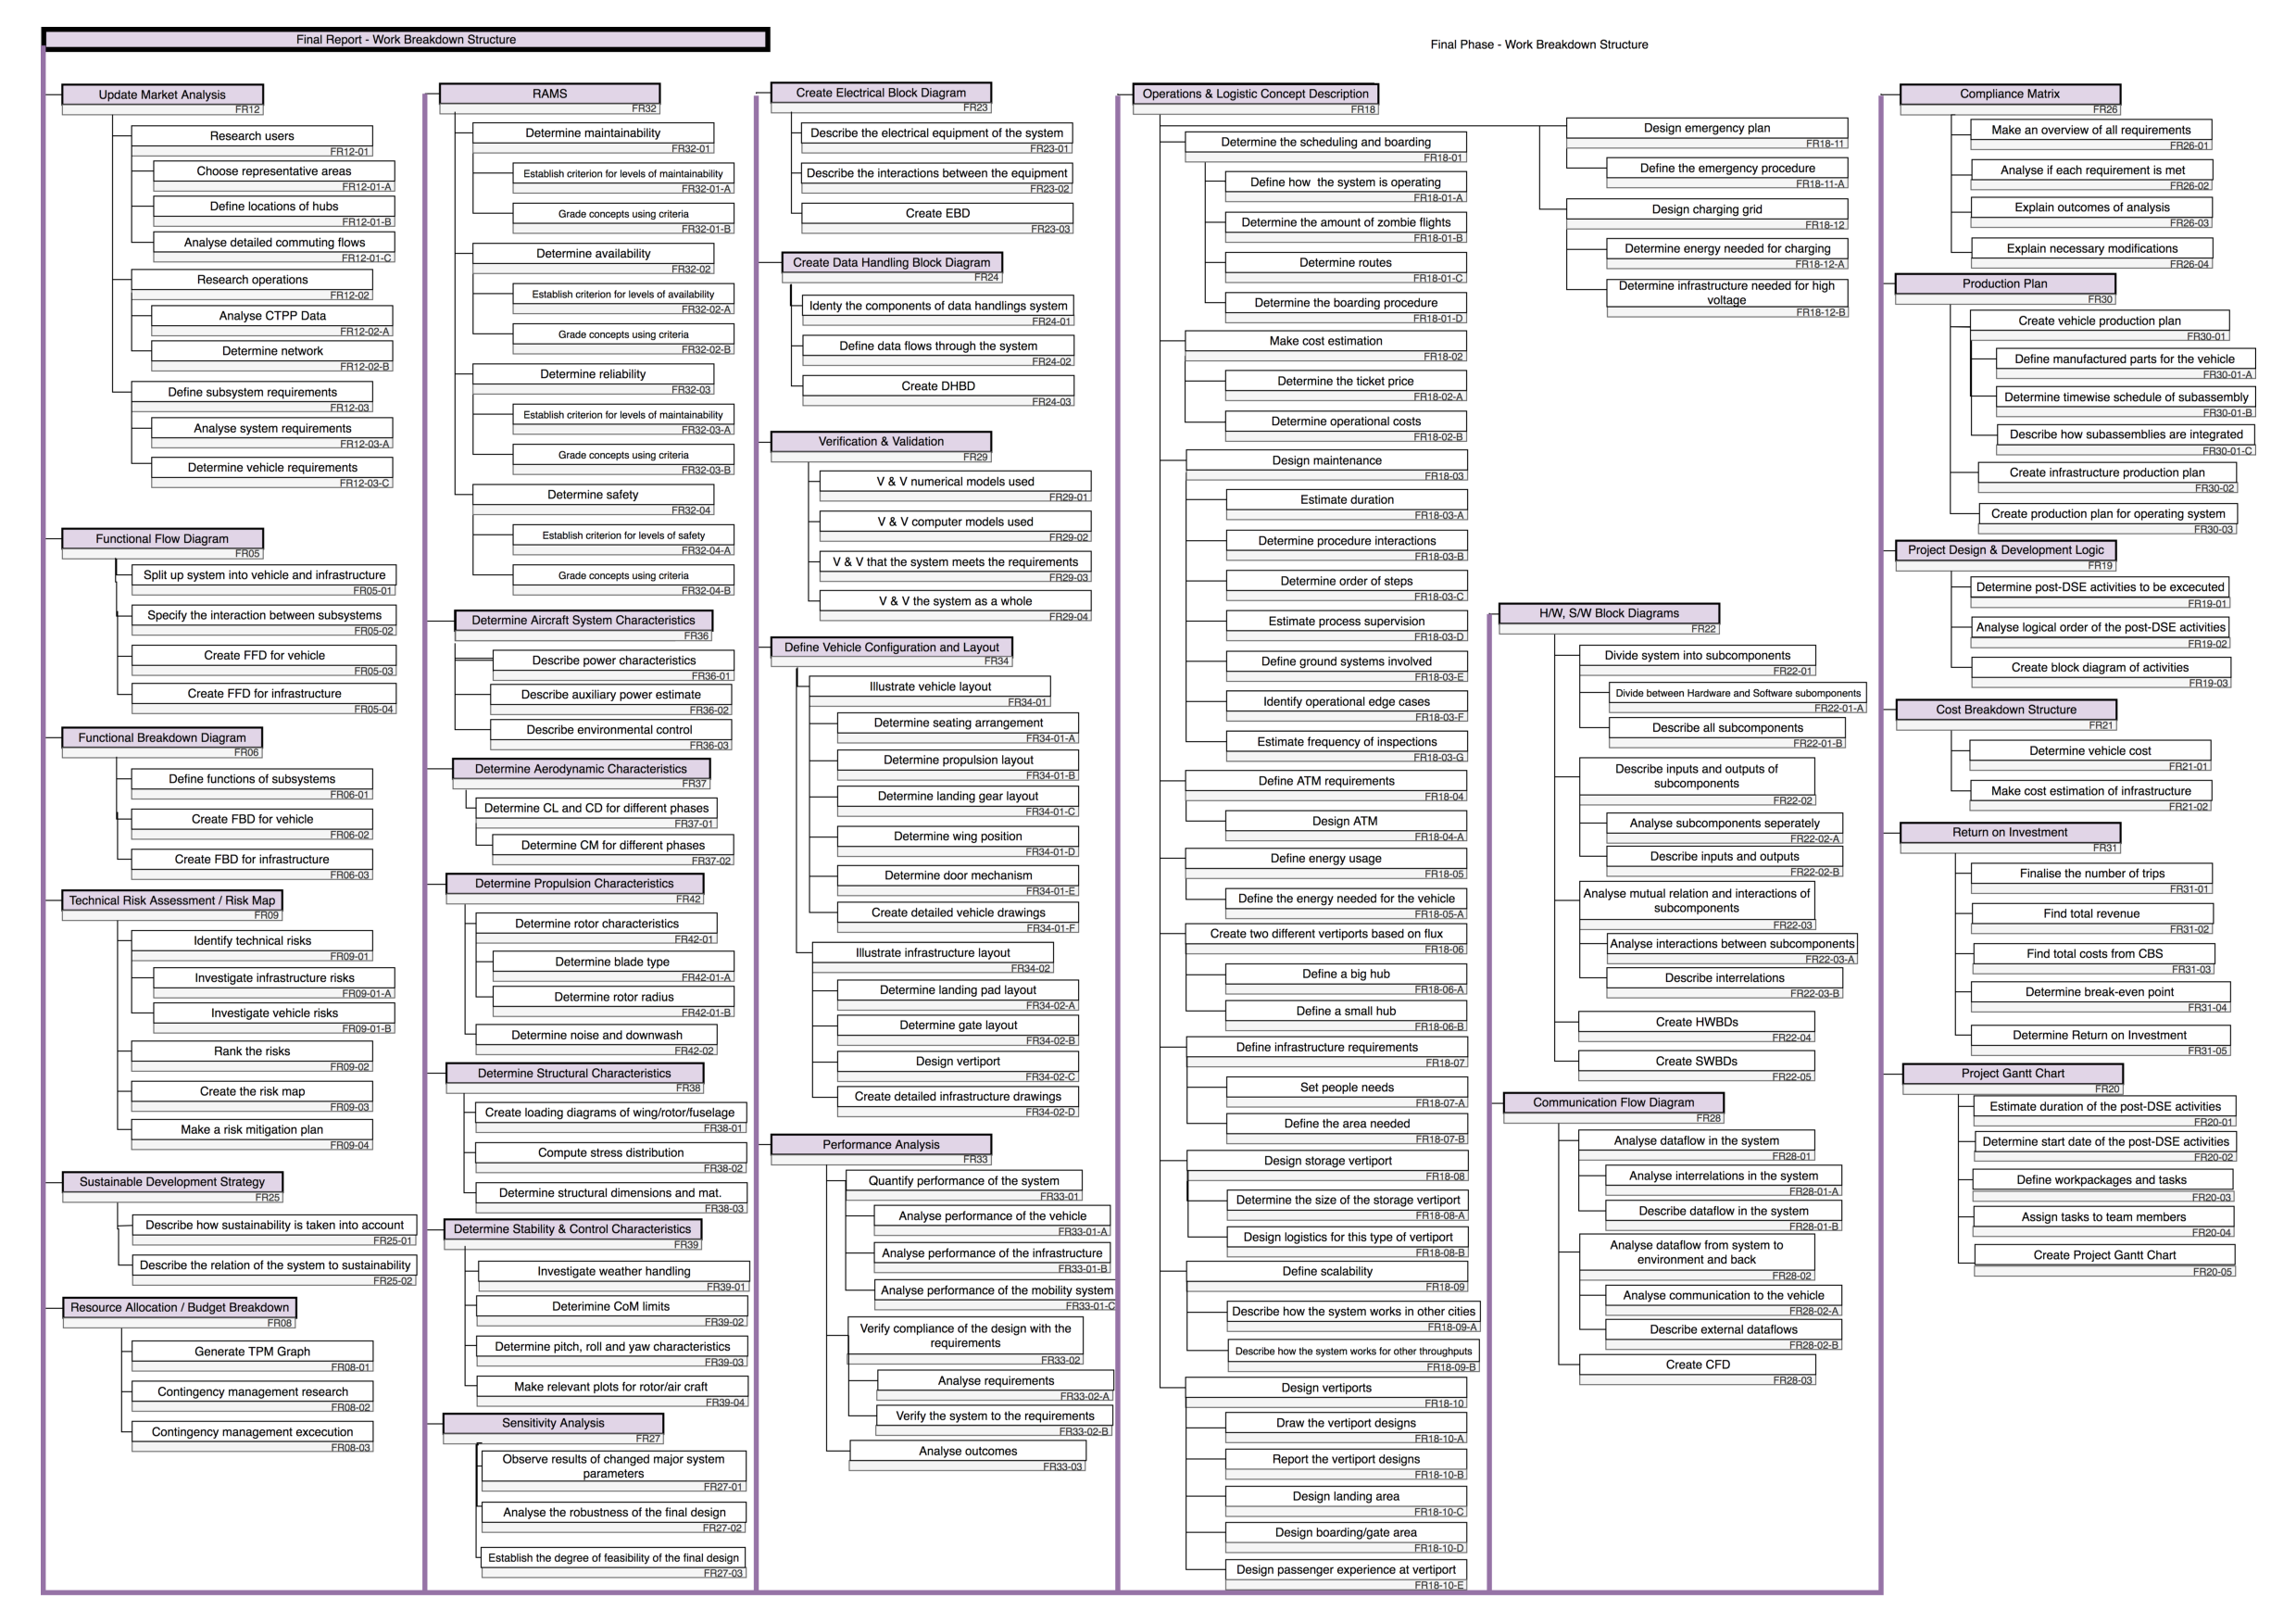
\includepdf[pages={1},fitpaper]{Figures/WBS_final.pdf}

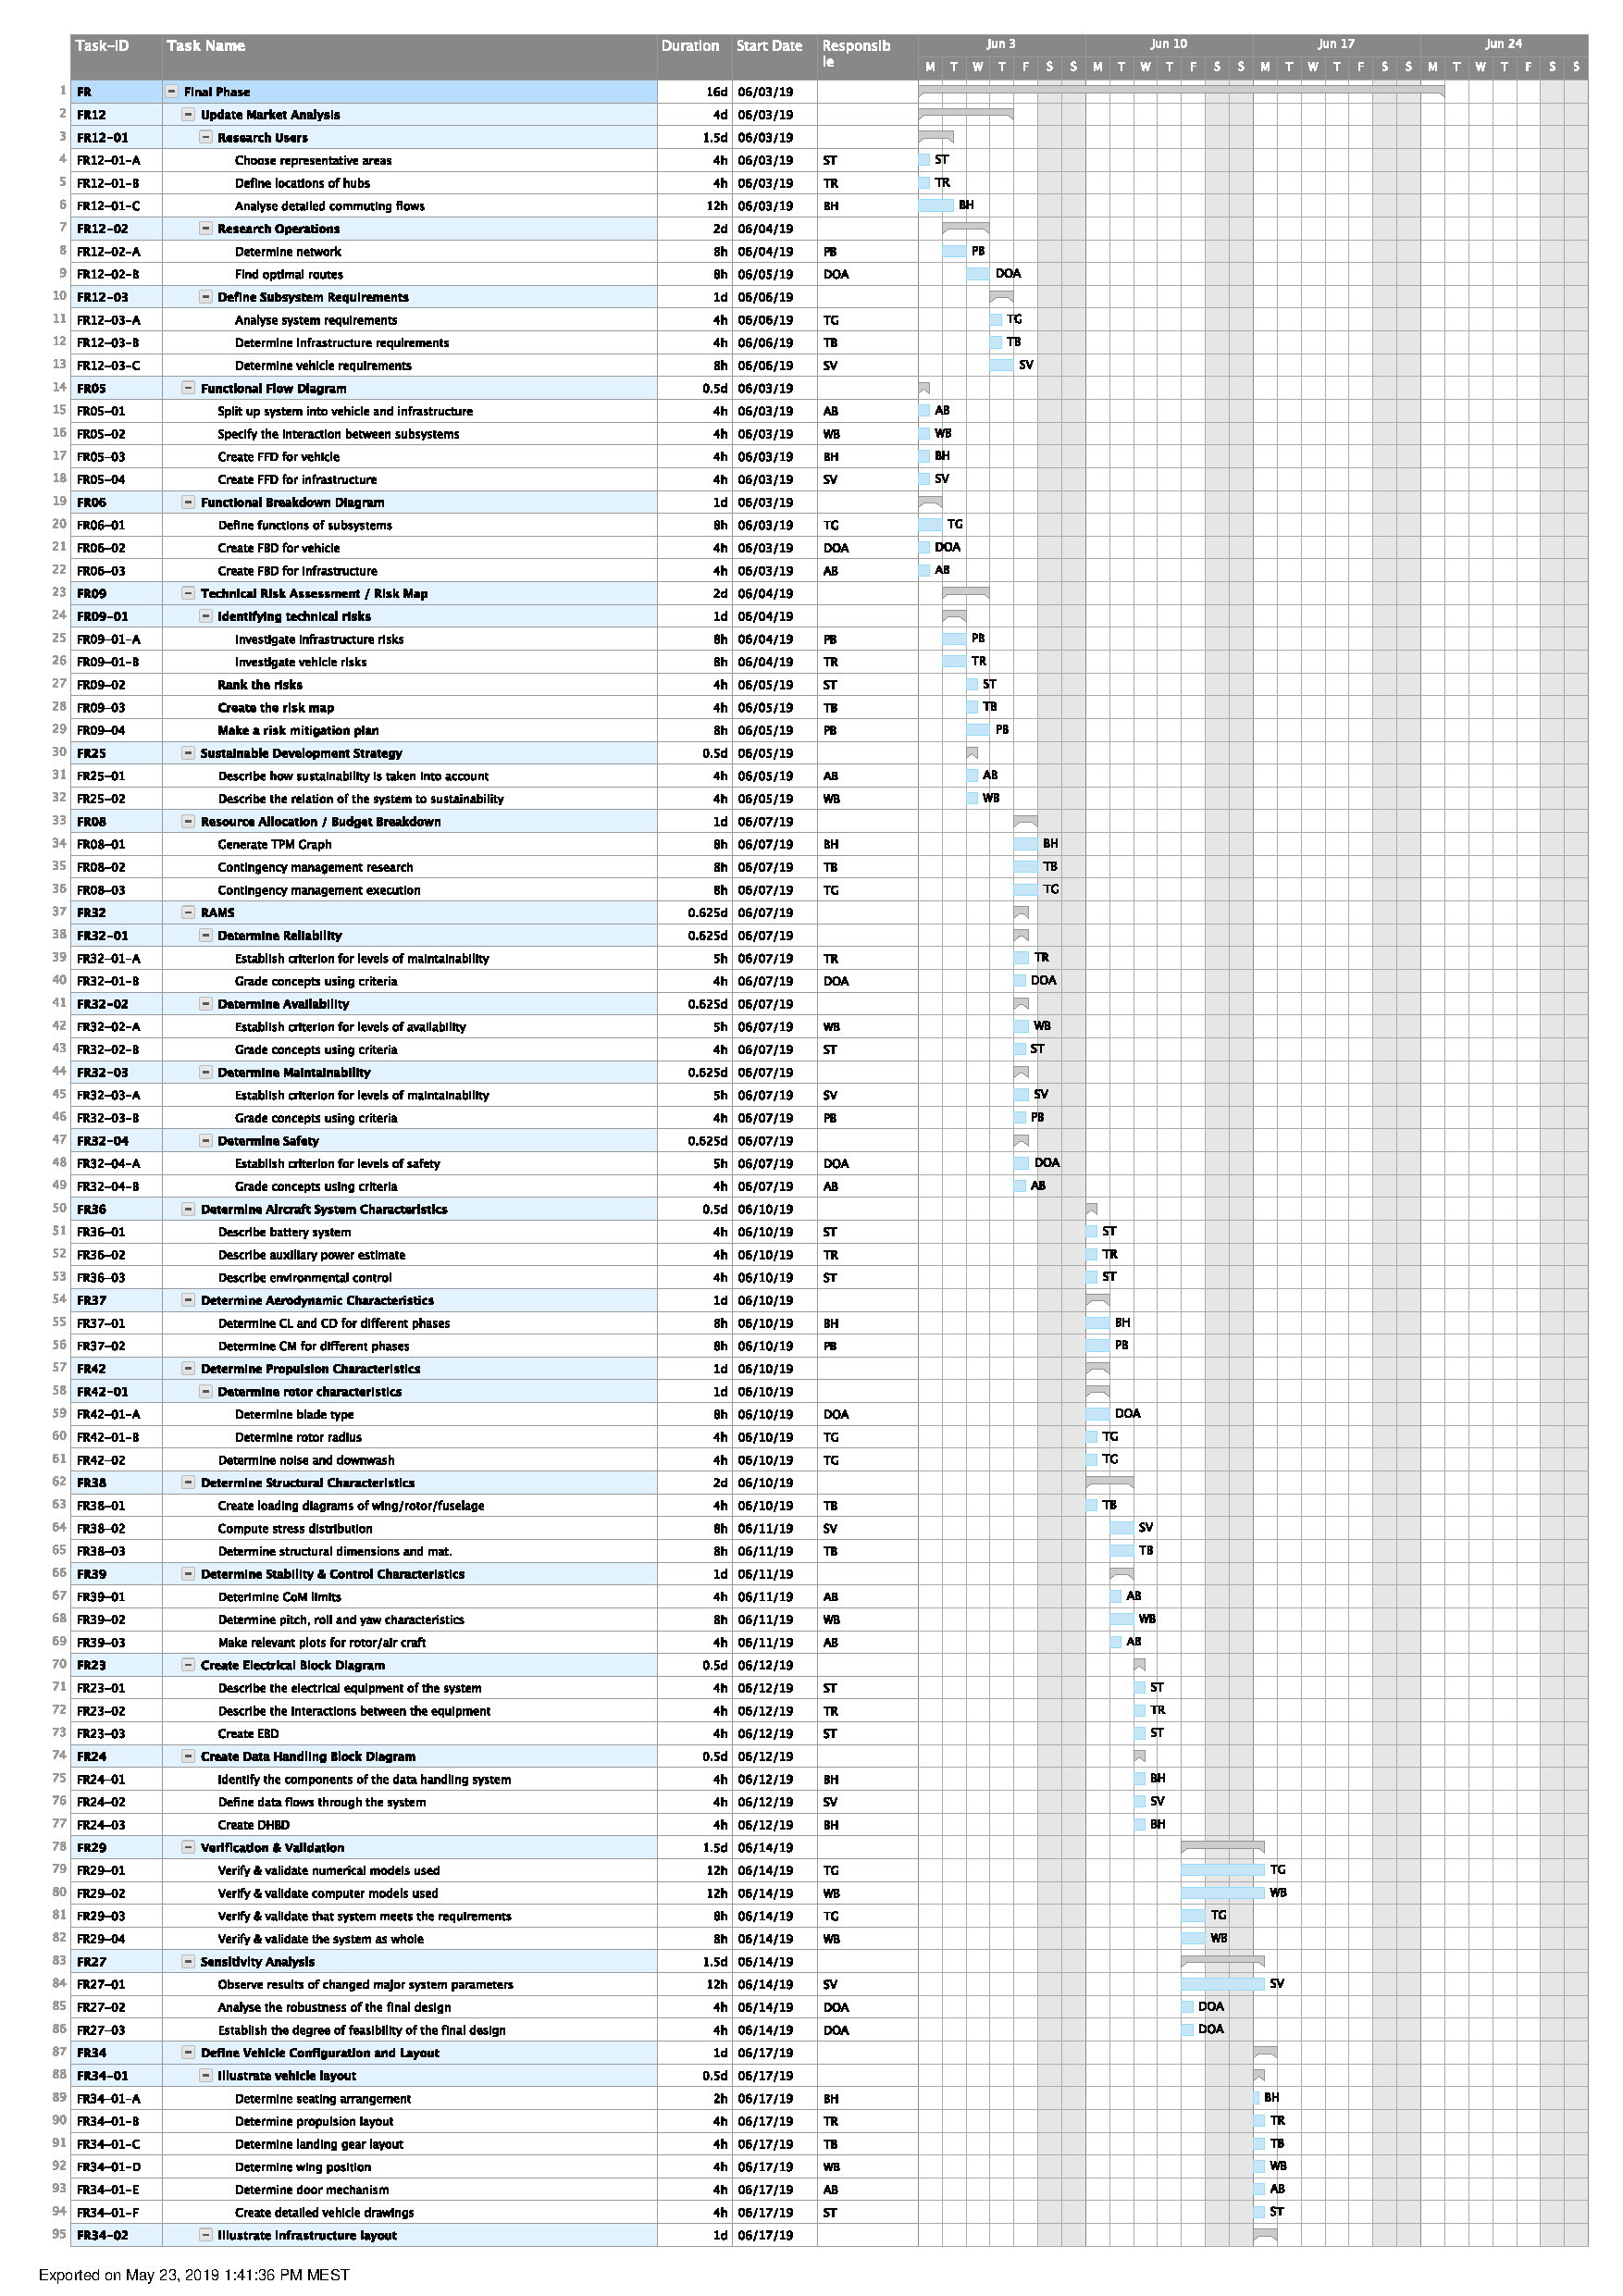
\includepdf[pages={1-2},fitpaper]{Figures/2019_05_23_Gantt_FR.pdf}